%
\chapter{Introducci\'{o}n}

\section{\textquestiondown Qu\'{e} es
%TCIMACRO{\TeXButton{TeX }{\TeX} }%
%BeginExpansion
\TeX
%EndExpansion
y
%TCIMACRO{\TeXButton{latex}{\LaTeX}}%
%BeginExpansion
\LaTeX
%EndExpansion
?}%

%TCIMACRO{\TeXButton{TeX }{\TeX} }%
%BeginExpansion
\TeX
%EndExpansion
\ es un sistema profesional de

composici\'{o}n tipogr\'{a}fica desarrollado por

Donald E. Knuth.%
%TCIMACRO{\FRAME{dhF}{1.3578in}{1.855in}{0pt}{}{}{don.jpg}%
%{\special{ language "Scientific Word";  type "GRAPHIC";
%maintain-aspect-ratio TRUE;  display "USEDEF";  valid_file "F";
%width 1.3578in;  height 1.855in;  depth 0pt;  original-width 1.9441in;
%original-height 2.6671in;  cropleft "0";  croptop "1";  cropright "1";
%cropbottom "0";  filename 'don.jpg';file-properties "XNPEU";}}}%
%BeginExpansion
\begin{center}
\includegraphics[
natheight=2.667100in,
natwidth=1.944100in,
height=1.855in,
width=1.3578in
]%
{don.jpg}%
\end{center}
%EndExpansion
%

%TCIMACRO{\TeXButton{TeX }{\TeX} }%
%BeginExpansion
\TeX
%EndExpansion
fu\'{e} dise\~{n}ado para producir documentos

(especialmente de matem\'{a}ticas) con la m\'{a}s

alta calidad de imprenta.y es la base sobre lo cu\'{a}l se construye todo.%

%TCIMACRO{\TeXButton{TeX }{\TeX} }%
%BeginExpansion
\TeX
%EndExpansion
\ se pronuncia ((Tej)) y la \'{u}ltima versi\'{o}n es la 3.14159%

%TCIMACRO{\TeXButton{latex}{\LaTeX} }%
%BeginExpansion
\LaTeX
%EndExpansion
\ es un sistema de macros, desarrollado

sobre
%TCIMACRO{\TeXButton{tex}{\TeX} }%
%BeginExpansion
\TeX
%EndExpansion
\ por Leslie Lamport, para facilitar su

uso por parte de los autores. se pronuncia (( La-Tej)) la versi\'{o}n actual
es
%TCIMACRO{\TeXButton{latex}{\LaTeX2$ \epsilon$} }%
%BeginExpansion
\LaTeXe
%EndExpansion
\ la cual se actualiza cada 6 meses%

%TCIMACRO{\FRAME{dhF}{3.4982in}{1.8152in}{0pt}{}{}{imprenta.jpg}%
%{\special{ language "Scientific Word";  type "GRAPHIC";
%maintain-aspect-ratio TRUE;  display "USEDEF";  valid_file "F";
%width 3.4982in;  height 1.8152in;  depth 0pt;  original-width 2.9758in;
%original-height 1.5316in;  cropleft "0";  croptop "1";  cropright "1";
%cropbottom "0";  filename \'imprenta.jpg';file-properties "XNPEU";}}}%
%BeginExpansion
\begin{center}
\includegraphics[
natheight=1.531600in,
natwidth=2.975800in,
height=1.8152in,
width=3.4982in
]%
{imprenta.jpg}%
\end{center}
%EndExpansion


\section{Word Vs
%TCIMACRO{\TeXButton{latex}{\LaTeX}}%
%BeginExpansion
\LaTeX
%EndExpansion
}

\bigskip
\begin{minipage}[t]{0.45\linewidth}
\begin{center}
Word
\end{center}
\begin{description}
\item[$\blacklozenge$] Wysiwyg
\item[$\blacklozenge$] Muy f\'{a}cil de usar
\item[$\blacklozenge$] Facilidades para insertar objetos
\item[$\blacklozenge$] Lento y malo para trabajar con f\'{o}rmulas
\item[$\blacklozenge$] \'Enfasis en dise\~{n}o
\item[$\blacklozenge$] Comercial
\end{description}
\end{minipage}%
%TCIMACRO{\TeXButton{latex}{\LaTeX}}%
%BeginExpansion
\hfill
\LaTeX
%EndExpansion
\begin{minipage}[t]{0.45\linewidth}
\begin{description}
\item[$\blacklozenge$] Preprosesado
\item[$\blacklozenge$] No es f\'{a}cil de usar
\item[$\blacklozenge$] Limitaciones por aceptar pocos formatos
\item[$\blacklozenge$] Excelente en el manejo de f\'{o}rmulas
\item[$\blacklozenge$] En contenido
\item[$\blacklozenge$] Gratis
\end{description}
\end{minipage}


\section{� Porqu\'{e} Usar
%TCIMACRO{\TeXButton{latex}{\LaTeX}}%
%BeginExpansion
\LaTeX
%EndExpansion
?}

\begin{description}
\item[$\spadesuit$] Produce documentos con calidad de imprenta.

\item[$\spadesuit$] Es utilizado por editoriales (Springer, Elsevier,. . . ),
revistas y congresos especializados.

\item[$\spadesuit$] Es una herramienta indispensable para f\'{\i}sicos y
matem\'{a}ticos, especialmente para investigadores.

\item[$\spadesuit$] Es una muy buena opci\'{o}n para escribir su tesis profesional.
\end{description}

\section{Filosof\'{\i}a de
%TCIMACRO{\TeXButton{latex}{\LaTeX}}%
%BeginExpansion
\LaTeX
%EndExpansion
}

\textquotedblleft El autor debe de preocuparse por el contenido de sus
documentos, y no por la apariencia que \'{e}stos tendr\'{a}n impresos en
papel.\textquotedblright\

En este tutorial veremos:

\begin{description}
\item[$\bigstar$] Comandos que definen unidades tem\'{a}ticas: t\'{\i}tulo,
secci\'{o}n, figuras, . . .

\item[$\bigstar$] No veremos comandos de formato: centrado, negritas, letra
grande, . . . \textexclamdown eso es tarea del dise\~{n}ador!
\end{description}

\section{Herramientas para trabajar con
%TCIMACRO{\TeXButton{latex}{\LaTeX}}%
%BeginExpansion
\LaTeX
%EndExpansion
}

\begin{description}
\item[$\bigstar$]
%TCIMACRO{\TeXButton{latex}{\LaTeX} }%
%BeginExpansion
\LaTeX
%EndExpansion
\ es un programa originario del sistema operativo Unix, pero existe una
versi\'{o}n para windows llamada MiKTeX, la cual funciona bajo DOS y no bajo
Windows .Este se consigue en \url{www.miktex.org} y su \'{u}ltima versi\'{o}n
es la 2.4.1461%
%TCIMACRO{\FRAME{dhF}{3.3174in}{2.5815in}{0pt}{}{}{tfz.png}%
%{\special{ language "Scientific Word";  type "GRAPHIC";
%maintain-aspect-ratio TRUE;  display "USEDEF";  valid_file "F";
%width 3.3174in;  height 2.5815in;  depth 0pt;  original-width 7.1866in;
%original-height 5.5798in;  cropleft "0";  croptop "1";  cropright "1";
%cropbottom "0";  filename 'tfz.png';file-properties "XNPEU";}}}%
%BeginExpansion
\begin{center}
\includegraphics[
natheight=5.579800in,
natwidth=7.186600in,
height=2.5815in,
width=3.3174in
]%
{tfz.png}%
\end{center}
%EndExpansion


\item[$\bigstar$] Como editor se puede usar cualquier editor de texto como el
Notepad o el Worpad, los cuales son accesorios de windows, pero existen varios
editores especializados

\begin{enumerate}
\item Uno muy bueno y adem\'{a}s gratis se llama TeXnicCenter el cual se
consigue en \url{www.toolscenter.org}%
%TCIMACRO{\FRAME{dhF}{3.7265in}{2.8029in}{0pt}{}{}{texniccenter.jpg}%
%{\special{ language "Scientific Word";  type "GRAPHIC";
%maintain-aspect-ratio TRUE;  display "USEDEF";  valid_file "F";
%width 3.7265in;  height 2.8029in;  depth 0pt;  original-width 10.6666in;
%original-height 8.0004in;  cropleft "0";  croptop "1";  cropright "1";
%cropbottom "0";  filename 'texniccenter.jpg';file-properties "XNPEU";}}}%
%BeginExpansion
\begin{center}
\includegraphics[
natheight=8.000400in,
natwidth=10.666600in,
height=2.8029in,
width=3.7265in
]%
{texniccenter.jpg}%
\end{center}
%EndExpansion
\item WinEdt, este es comercial , pero es el mejor, adem\'{a}s no es caro se
consigue en \url{www.winedt.com}%
%TCIMACRO{\FRAME{dhF}{3.8657in}{2.9075in}{0pt}{}{}{winedt.jpg}%
%{\special{ language "Scientific Word";  type "GRAPHIC";
%maintain-aspect-ratio TRUE;  display "USEDEF";  valid_file "F";
%width 3.8657in;  height 2.9075in;  depth 0pt;  original-width 10.6666in;
%original-height 8.0004in;  cropleft "0";  croptop "1";  cropright "1";
%cropbottom "0";  filename 'winedt.jpg';file-properties "XNPEU";}}}%
%BeginExpansion
\begin{center}
\includegraphics[
natheight=8.000400in,
natwidth=10.666600in,
height=2.9075in,
width=3.8657in
]%
{winedt.jpg}%
\end{center}
%EndExpansion
%\newline
\item Lyx Es apenas un proyecto , pero a pesar de eso es bueno y adem\'{a}s
gratis se consigue en \url{www.wingnu.org}%
%TCIMACRO{\FRAME{dhF}{3.7265in}{2.6705in}{0pt}{}{}{lyx2.jpg}%
%{\special{ language "Scientific Word";  type "GRAPHIC";
%maintain-aspect-ratio TRUE;  display "USEDEF";  valid_file "F";
%width 3.7265in;  height 2.6705in;  depth 0pt;  original-width 7.2921in;
%original-height 5.2088in;  cropleft "0";  croptop "1";  cropright "1";
%cropbottom "0";  filename 'lyx2.jpg';file-properties "XNPEU";}}}%
%BeginExpansion
\begin{center}
\includegraphics[
natheight=5.208800in,
natwidth=7.292100in,
height=2.6705in,
width=3.7265in
]%
{lyx2.jpg}%
\end{center}
%EndExpansion
\newline\newline

\item Scientific Work Place 5.0. Este es un super programa, mucho mejor que
Word , s\'{o}lo le falta una herramienta para realizar dibujos. se consigue en
\url{www.tcisoft.com}%
%TCIMACRO{\FRAME{dhF}{4.0387in}{3.0381in}{0pt}{}{}{swp1.jpg}%
%{\special{ language "Scientific Word";  type "GRAPHIC";
%maintain-aspect-ratio TRUE;  display "USEDEF";  valid_file "F";
%width 4.0387in;  height 3.0381in;  depth 0pt;  original-width 10.6666in;
%original-height 8.0004in;  cropleft "0";  croptop "1";  cropright "1";
%cropbottom "0";  filename 'swp1.jpg';file-properties "XNPEU";}}}%
%BeginExpansion
\begin{center}
\includegraphics[
natheight=8.000400in,
natwidth=10.666600in,
height=3.0381in,
width=4.0387in
]%
{swp1.jpg}%
\end{center}
%EndExpansion


\item Hay tres herramientas adicionales para completar la plataforma y
son\newline Adobe Acrobat Reader y Ghost-Ghost view,\newline Estas
herramientas hay que instalarlas de primero para que MiKTeX y los
editores las reconozcan.
\end{enumerate}
\end{description}

\chapter{Edici\'{o}n B\'{a}sica}

Ordenes de TEX/ LATEX:

\begin{description}
\item[$\blacksquare$] Comienzan por una barra invertida: ((%
%TCIMACRO{\TEXTsymbol{\backslash}}%
%BeginExpansion
$\backslash$%
%EndExpansion
))

\item[$\blacksquare$] Distinguen may\'{u}sculas-min\'{u}sculas

\item[$\blacksquare$] $\ $Dos tipos:
\end{description}

1. con letras s\'{o}lo (pueden ser varias)

2. con car\'{a}cter especial (uno s\'{o}lo)

\begin{description}
\item[$\blacksquare$]  TEX ignora los espacios en blanco justo despu\'{e}s de
un mandato: para tenerlos en cuenta, escribir \{\}

\item[$\blacksquare$] Par\'{a}metros: [opcionales] y \{obligatorios\}
\end{description}

\subsection{Ejemplos de comandos}

\begin{description}
\item[$\spadesuit$] Comentarios: a partir de signo \%, son ignorados
\end{description}

Veamos algunas ordenes:

\TeX \LaTeX      %  \\es una orden de tipo 2


\begin{verbatim}
\TeX \LaTeX      %  \\es una orden de tipo 2
\end{verbatim}

\TeX {}\LaTeX     \\[2ex]

\today\\[4ex]
\begin{verbatim}

\today  \\[4ex]
\end{verbatim}



\textbf{texto resaltado}


\begin{verbatim}
\emph {texto resaltado}
\end{verbatim}

\subsection{Caracteres especiales}

Los caracteres con un significado especial, si se desean transcribir hay que
indicarlo de alguna manera:
\begin{verbatim}
$ & % # _ { } ~^\
\$ \& \% \# \_ \{ \}
\\  \verb+ ~ ^ \+
\end{verbatim}




\section{Mi primer documento}
\subsection{Estructura de un fichero de entrada}

Cuando \LaTeXe{} procesa un fichero de entrada, espera de \'el que
siga una determinada \wi{estructura}. Todo fichero de entrada debe
comenzar con la orden
\begin{code}
\verb|\documentclass{...}|
\end{code}
Esto indica qu\\'e tipo de documento es el que se pretende crear.
Tras esto, se pueden incluir \'ordenes que influir\'an sobre el
estilo del documento entero, o puede cargar \wi{paquete}s que
a~nadir\'an nuevas propiedades al sistema de \LaTeX. Para cargar
uno de estos paquetes se usar\'a la instrucci\'on
\begin{code}
\verb|\usepackage{...}|
\end{code}

Cuando todo el trabajo de configuraci\'on est\\'e
realizado\footnote{El
  \'area entre \texttt{\bs documentclass} y \texttt{\bs
    begin$\mathtt{\{}$document$\mathtt{\}}$} se llama
  \emph{\wi{pre\'ambulo}}.} entonces comienza el cuerpo del texto con
la instrucci\'on
\begin{code}
\verb|\begin{document}|
\end{code}

A partir de entonces se introducir\'a el texto mezclado con algunas
instrucciones \'utiles de \LaTeX. Al finalizar el documento debe
ponerse la orden
\begin{code}
\verb|\end{document}|
\end{code}
LaTeX{} ingorar\'a cualquier cosa que se ponga tras esta
instrucci\'on.

La figura~\ref{mini} muestra el contenido m\'inimo de un fichero de
\LaTeXe. En la figura~\ref{document} se expone un \wi{fichero de
  entrada} algo m\'as complejo.

\begin{figure}[!bp]
\begin{verbatim}
\documentclass{article}
\begin{document}
Lo peque~no es bello.
\end{document}
\end{verbatim}
\caption{Un fichero m\'inimo de \LaTeX} \label{mini}
\end{figure}

\begin{figure}[!bp]
\begin{verbatim}
\documentclass[a4paper,11pt]{article}
\usepackage{latexsym}
\usepackage[activeacute,spanish]{babel}
\author{H.~Partl}
\title{Minimizando}
\frenchspacing
\begin{document}
\maketitle \tableofcontents
\section{Inicio}
Bien\ldots{} y aqu\'i comienza
mi art\'iculo tan estupendo.
\section{Fin}
\ldots{} y aqu\'i acaba.
\end{document}
\end{verbatim}
\caption{Ejemplo para un art\'iculo cient\'ifico en espa~nol.}
\label{document}
\end{figure}

\section{El formato del documento}

\subsection{Clases de documentos}\label{sec:documentclass}

Cuando procesa un fichero de entrada, lo primero que necesita
saber \LaTeX{} es el tipo de documento que el autor quiere crear.
Esto se indica con la instrucci\'on \ci{documentclass}.
\begin{command}
\ci{documentclass}\verb|[|\emph{opciones}\verb|]{|\emph{clase}\verb|}|
\end{command}
\noindent En este caso, la \emph{clase} indica el tipo de
documento que se crear\'a. En la tabla~\ref{documentclasses} se
muestran las clases de documento que se explican en esta
introducci\'on. La distribuci\'on de \LaTeXe{} proporciona m\'as
clases para otros documentos, como cartas y transparencias. El
par\'ametro de \emph{\wi{opciones}} personaliza el comportamiento
de la clase de documento elegida. Las opciones se deben separar
con comas. En la tabla~\ref{options} se indican las opciones m\'as
comunes de las clases de documento est\'andares.


\begin{table}[!bp]
\caption{Clases de documentos} \label{documentclasses}
\begin{description}

\item [\normalfont\texttt{article}] para art\'iculos de revistas
  especializadas, ponencias, trabajos de pr\'acticas de formaci\'on,
  trabajos de seminarios, informes peque'nos, solicitudes,
  dict\'amenes, descripciones de programas, invitaciones y muchos
  otros.\index{articulo@art\'iculo}%
\index{clase \texttt{article}@clase article}
\item [\normalfont\texttt{report}] para informes mayores que constan
  de m\'as de un cap\'itulo, proyectos fin de carrera, tesis doctorales,
  libros peque'nos, disertaciones, guiones y
  similares.\index{informe}\index{clase \texttt{report}@clase report}
\item [\normalfont\texttt{book}] para libros de
  verdad\index{libro}\index{clase \texttt{book}@clase book}
\item [\normalfont\texttt{slide}] para transparencias. Esta clase emplea
  tipos grandes \textsf{sans serif}.
  \index{transparencias}\index{clase \texttt{slide}@clase slide}
\end{description}
\end{table}

\begin{table}[!bp]
\caption{Opciones de clases de documento} \label{options}
\begin{flushleft}
\begin{description}
\item[\normalfont\texttt{10pt}, \texttt{11pt}, \texttt{12pt}] \quad
  Establecen el tama~no (cuerpo) para los tipos. Si no se especifica
  ninguna opci\'on, se toma \texttt{10pt}.\index{tama~no de los
    tipos!del documento}
\item[\normalfont\texttt{a4paper}, \texttt{letterpaper}, \ldots] \quad
  Define el tama~no del papel. Si no se indica nada, se toma
  \texttt{letterpaper}. Aparte de \\'este se puede elegir
  \texttt{a5paper}, \texttt{b5paper}, \texttt{executivepaper} y
  \texttt{legalpaper}. \index{papel legal} \index{tama~no del
    papel}\index{papel DIN-A4} \index{papel de carta} \index{papel DIN-A5}\
  \index{papel DIN-B5} \index{papel ejecutivo}

\item[\normalfont\texttt{fleqn}] \quad Dispone las ecuaciones hacia la
  izquierda en vez de centradas.

\item[\normalfont\texttt{leqno}] \quad Coloca el n\'umero de las
  ecuaciones a la izquierda en vez de a la derecha.
  \vspace{5cm}

\item[\normalfont\texttt{titlepage}, \texttt{notitlepage}] \quad
  Indica si se debe comenzar una p\'agina nueva tras el \wi{t\'itulo del
    documento} o no. Si no se indica otra cosa, la clase
  \texttt{article} no comienza una p\'agina nueva, mientras que \texttt{report}
  y \texttt{book} s\'i.\index{titlepage@\texttt{titlepage}}

\item[\normalfont\texttt{twocolumn}] \quad Le dice a \LaTeX{} que
  componga el documento en \wi{dos columnas}.

\item[\normalfont\texttt{twoside, oneside}] \quad Especifica si se
  debe generar el documento a una o a dos caras.  En caso de no
  indicarse otra cosa, las clases \texttt{article} y \texttt{report}
  son a una cara y la clase \texttt{book} es a dos.

\item[\normalfont\texttt{openright, openany}] \quad Hace que los
  cap\'itulos comienzen o bien s\'olo en p\'aginas a la derecha, o bien
  en la pr\'oxima que est\\'e disponible. Esto no funciona con la clase
  \texttt{article}, ya que en esta clase no existen cap\'itulos. De
  modo predeterminado, la clase \texttt{report} comienza los
  cap\'itulos en la pr\'oxima p\'agina disponible y la clase
  \texttt{book} las comienza en las p\'aginas a la derecha.
\end{description}
\end{flushleft}
\end{table}

Por ejemplo: un fichero de entrada para un documento de \LaTeX{}
podr\'ia comenzar con
\begin{code}
\ci{documentclass}\verb|[11pt,twoside,a4paper]{article}|
\end{code}
Esto le indica a \LaTeX{} que componga el documento como un
\emph{art\'iculo} utilizando tipos del cuerpo 11, y que produzca un
formato para impresi\'on a \emph{doble cara} en \emph{papel
DIN-A4}.

\pagebreak[2]
\subsection{Paquetes}
\index{paquete} Mientras escribe su documento, probablemente se
encontrar\'a en situaciones donde el \LaTeX{} b\'asico no basta para
solucionar su problema. Si desea incluir \wi{gr\'aficos}, \wi{texto
en
  color} o el c\'odigo fuente de un fichero, necesita mejorar las
capacidades de \LaTeX. Tales mejoras se realizan con ayuda de los
llamados \emph{paquetes.} Los paquetes se activan con la orden
\begin{command}
\ci{usepackage}\verb|[|\emph{opciones}\verb|]{|\emph{paquete}\verb|}|
\end{command}
\noindent donde \emph{paquete} es el nombre del paquete y
\emph{opciones} es una lista palabras clave que activan funciones
especiales del paquete, a las que \LaTeX{} les a~nade las opciones
que previamente se hayan indicado en la orden
\verb|\documentclass|. Algunos paquetes vienen con la
distribuci\'on b\'asica de \LaTeXe{} (v\\'ease la
tabla~\ref{packages}). Otros se proporcionan por separado. En la
\guia{} puede encontrar m\'as informaci\'on sobre los paquetes
disponibles en su instalaci\'on local. La fuente principal de
informaci\'on sobre \LaTeX{} es \companion. Contiene descripciones
de cientos de paquetes, as\'i como informaci\'on sobre c\'omo
escribir sus propias extensiones a \LaTeXe.

\begin{table}[!hbp]
\caption{Algunos paquetes distribuidos con \LaTeX}
\label{packages}
\begin{description}
\item[\normalfont\pai{doc}] Permite la documentaci\'on de paquetes y
  otros ficheros de \LaTeX.\\ Se describe en \texttt{doc.dtx} y en
  \companion.

\item[\normalfont\pai{exscale}] Proporciona versiones escaladas de
  los tipos adicionales para matem\'aticas.\\
 Descrito en \texttt{ltexscale.dtx}.

\item[\normalfont\pai{fontenc}] Especifica qu\\'e \wi{codificaci\'on de
    tipo} debe usar \LaTeX.\\ Descrito en \texttt{ltoutenc.dtx}.
    \vspace{5cm}

\item[\normalfont\pai{ifthen}] Proporciona instrucciones de la forma\\
  `si\ldots{} entonces\ldots{} si no\ldots'\\ Descrito en
  \texttt{ifthen.dtx} y en \companion.

\item[\normalfont\pai{latexsym}] Para que \LaTeX{} acceda al tipo
  de s\'imbolos, se debe usar el paquete \texttt{latexsym}.\\ Descrito
  en \texttt{latexsym.dtx} y en \companion.

\item[\normalfont\pai{makeidx}] Proporciona instrucciones para
  producir \'indices de materias.\\ Descrito en el
  apartado~\ref{sec:indexing} y en \companion.

\item[\normalfont\pai{syntonly}] Procesa un documento sin
  componerlo.\\ Se describe en \texttt{syntonly.dtx} y en \companion.
  Es \'util para la verificaci\'on r\'apida de errores.

\item[\normalfont\pai{inputenc}] Permite la especificaci\'on de una
  codificaci\'on de entrada como ASCII (con la opci\'on \pai{ascii}),
  ISO Latin-1 (con la opci\'on \pai{latin1}), ISO Latin-2 (con la
  opci\'on \pai{latin2}), p\'aginas de c\'odigo de 437/850 IBM (con las
  opciones \pai{cp437} y \pai{cp580}, respectivamente), Apple
  Macintosh (con la opci\'on \pai{applemac}), Next (con la opci\'on
  \pai{next}), ANSI-Windows (con la opci\'on \pai{ansinew}) o una
  definida por el usuario.  Descrito en \texttt{inputenc.dtx}.

\end{description}
\end{table}

\clearpage
%
% Puntero a informaci\'on de los paquetes
%

\subsection{Estilo de p\'agina}

Con \LaTeX{} existen tres combinaciones predefinidas de
\wi{cabeceras} y \wi{pies de p\'agina}, a las que se llaman estilos
de p\'agina.\index{estilo de pagina@estilo de p\'agina} El
par\'ametro \emph{estilo} de la instrucci\'on
\index{estilo de pagina@estilo de p\'agina!plain@\texttt{plain}}%
\index{plain@\texttt{plain}}%
\index{estilo de pagina@estilo de p\'agina!headings@\texttt{headings}}%
\index{headings@\texttt{headings}}%
\index{estilo de pagina@estilo de p\'agina!empty@\texttt{empty}}%
\index{empty@\texttt{empty}}%
\begin{command}
\ci{pagestyle}\verb|{|\emph{estilo}\verb|}|
\end{command}
\noindent define cu\'al emplearse. La tabla~\ref{pagestyle} muestra
los estilos de p\'agina predefinidos.

\begin{table}[!hbp]
\caption{Estilos de p\'agina predefinidos en \LaTeX}
\label{pagestyle}
\begin{description}

\item[\normalfont\texttt{plain}] imprime los n\'umeros de p\'agina en el
  centro del pie de las p\'aginas. Este es el estilo de p\'agina que se
  toma si no se indica ning\'un otro.

\item[\normalfont\texttt{headings}] en la cabecera de cada p\'agina
  imprime el cap\'itulo que se est\'a procesando y el n\'umero de
  p\'agina, mientras que el pie est\'a vac\'io. (Este estilo es similar
  al empleado en este documento).

\item[\normalfont\texttt{empty}] deja tanto la cabecera como el pie
  de las p\'aginas vac\'ios.

\end{description}

\end{table}

Es posible cambiar el estilo de p\'agina de la p\'agina actual con
la instrucci\'on
\begin{command}
\ci{thispagestyle}\verb|{|\emph{estilo}\verb|}|
\end{command}
En \companion{} hay una descripci\'on de c\'omo crear sus propias
cabeceras y pies de p\'agina.
%
% Puntero a la descripci\'on del paquete fancyhdr
%
% Informaci\'on sobre la numeraci\'on de p\'aginas, ...
% \pagenumbering

\section{Proyectos grandes}

Cuando trabaje con documentos grandes, podr\'ia, si lo desea,
dividir el fichero de entrada en varias partes. \LaTeX{} tiene dos
instrucciones que le ayudan a realizar esto.

\begin{command}
\ci{include}\verb|{|\emph{fichero}\verb|}|
\end{command}
\noindent se puede utilizar en el cuerpo del documento para
introducir el contenido de otro fichero. En este caso, \LaTeX{}
comenzar\'a una p\'agina nueva antes de procesar el texto del
\emph{fichero}.

La segunda instrucci\'on s\'olo puede ser empleada en el pre\'ambulo.
Permite indicarle a \LaTeX{} que s\'olo tome la entrada de algunos
ficheros de los indicados con \verb|\include|.

\begin{command}
\ci{includeonly}\verb|{|\emph{fichero}\verb|,|\emph{fichero}%
\verb|,|\ldots\verb|}|
\end{command}

Una vez que esta instrucci\'on se ejecute en el pre\'ambulo del
documento, s\'olo se procesar\'an las instrucciones \ci{include} con
los ficheros indicados en el argumento de la orden
\ci{includeonly}. Observe que no hay espacios entre los nombres de
los ficheros y las comas.
\section{resumen}
Todo documento en
%TCIMACRO{\TeXButton{latex}{\LaTeX} }%
%BeginExpansion
\LaTeX
%EndExpansion
est\'{a} compuesto de dos partes

\begin{description}
\item[$\Diamond$] El preambulo :\newline En esta parte de colocan las ordenes
globale spara el documento, adem\'{a}s de los paquetes de
%TCIMACRO{\TeXButton{latex}{\LaTeX} }%
%BeginExpansion
\LaTeX
%EndExpansion
que se usar\'{a}n

\item[$\Diamond$] El Body, este est\'{a} dividido a su vez entres parte el
Front matter, main matter y el back matter
\end{description}

Para empezar explicaremos como se dise\~{n}a un art\'{\i}culo

\begin{description}
\item[$\blacksquare$] Se escribe el c\'{o}digo\end{description}
\begin{verbatim}
\documentclass[a4paper]{article}
\usepackage[spanish,activeacute]{babel}
\author {Pon tu nombre aqu\'{\i}}
\title{Mi Primer Documento}
\begin{document}
\maketitle
Hola . Este es mi primer documento .
\end{document}
\end{verbatim}

\begin{description}
\item[$\blacksquare$] Se realiza el proceso de compilaci\'{o}n

\begin{description}
\item[$\clubsuit$] Compilar:
\end{description}

\item >latex archivo.tex

\begin{description}
\item[$\clubsuit$] Pre-visualizar:
\end{description}

\item >xdvi archivo.dvi
\end{description}

$\clubsuit$\textbf{Generar Post-Script:}

\begin{description}
\item >dvips archivo.dvi -o archivo.ps

\begin{description}
\item[$\clubsuit$] Imprimir:
\end{description}

\item >lpr -Plaser1sala4 archivo.ps
\end{description}
\begin{figure}
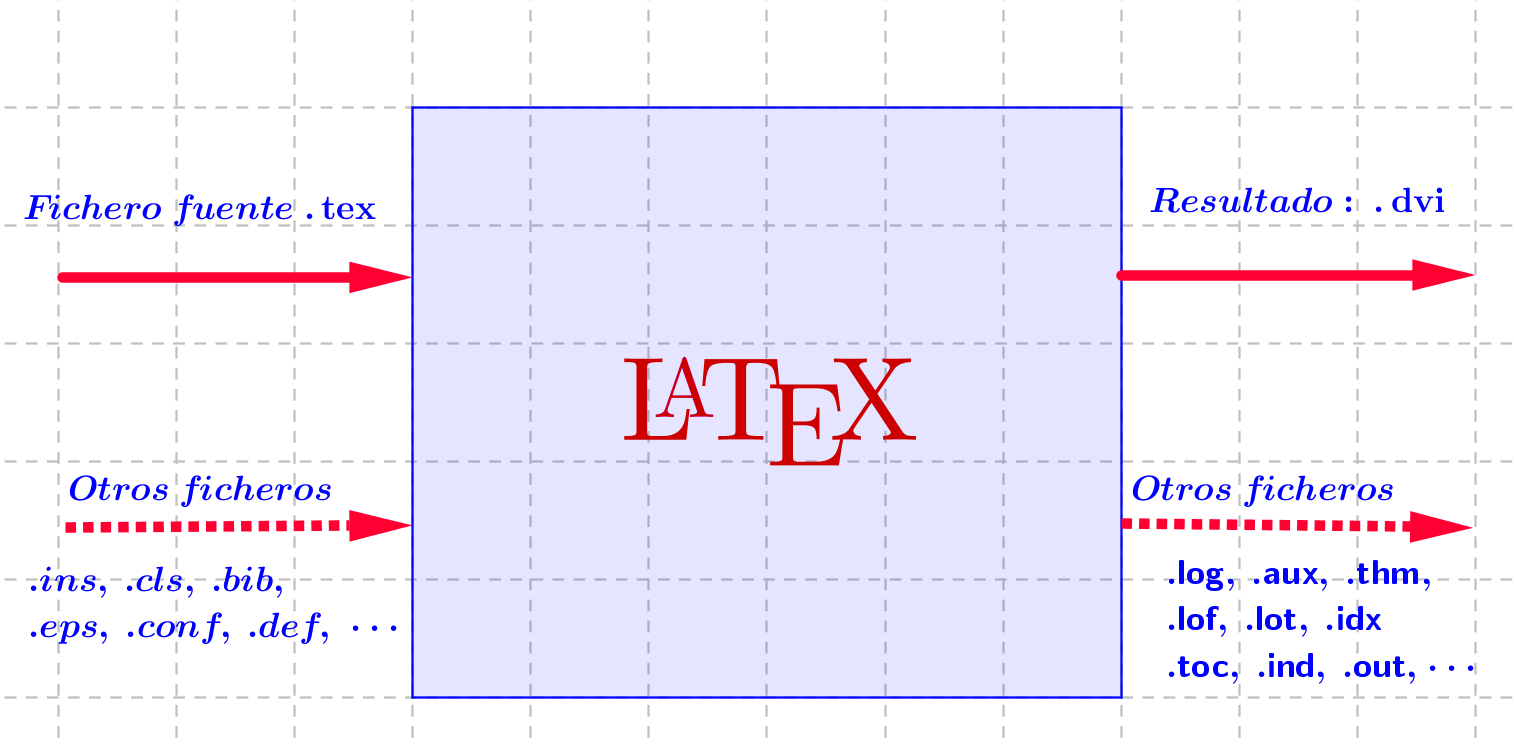
\includegraphics[scale=0.1]{diagrama.png}
\end{figure}

\section{Reglas generales}

\begin{description}
\item[$\clubsuit$] Usar espacios para separar palabras.

\item Un espacio vale igual que mil.

\begin{description}
\item[$\clubsuit$] Los fines de linea sencillos no valen.

\item[$\clubsuit$] Usar l�neas vac\'{\i}as para separar p\'{a}rrafos.
\end{description}
\end{description}

Una linea vac\'{\i}a vale igual que mil.

\begin{description}
\item
\begin{description}
\item[$\clubsuit$] El espaciado y las sangr\'{\i}as son trabajo de
\end{description}

\item LATEX, y lo sabe hacer muy bien.

\begin{description}
\item[$\clubsuit$] No forzar espacios ni cortes de l\'{\i}nea.
\end{description}
\end{description}

\subsection{Ejemplo 1}
\begin{verbatim}
\begin{document}
\maketitle Este es el primer p�rrafo ,
y esta sigue
siendo par te del primer p �rrafo
 Este ya es e l segundo p�rrafo .
%y esto es un comentario
Aqu� puedes e s c r i b i r m�s .
\ end{ document }

\end{verbatim}

\subsection{Ejemplo 2}
\begin{verbatim}

\begin{document}
\maketitle Este es un ejemplo con un
p � r ra fo m\'{a}s grande
que , por c i e r t o , tambi \'{e}n
es mucho m\'{a}s i n te re sa
n te . Recuerda que un p\'{a} r ra fo
debe expresar una idea
completa y coherente . Justo como este
 p \'{a} r ra fo que nos ha
servido como un ejemplo genial . Observa
que los p \'{a} r ra fo s
en \ LaTeX { } forman l a unidad
e s t r u c t u r a l m\'{a}s
peque~na dent ro de los documentos .
 Recuerda que es tu responsabilidad
  e l contenido de estos
p�rrafos , y de \ LaTeX { } e l
que se vean boni tos . \ end{ document }
\end{verbatim}

\subsection{Acentos}

La opci\'{o}n activeacute de babel permite

usar acentos cortos: \'{a}, \'{a}, \'{a}, \~{n}, etc.

Los acentos cortos no funcionan en el

pre\'{a}mbulo, all\'{\i} hay que usar acentos largos:

\'{a}
%TCIMACRO{\TEXTsymbol{\backslash}}%
%BeginExpansion
$\backslash$%
%EndExpansion
\'a \'{o}
%TCIMACRO{\TEXTsymbol{\backslash}}%
%BeginExpansion
$\backslash$%
%EndExpansion
\'o

\'{e}
%TCIMACRO{\TEXTsymbol{\backslash}}%
%BeginExpansion
$\backslash$%
%EndExpansion
\'e \'{u}
%TCIMACRO{\TEXTsymbol{\backslash}}%
%BeginExpansion
$\backslash$%
%EndExpansion
\'u

\'{\i}
%TCIMACRO{\TEXTsymbol{\backslash}}%
%BeginExpansion
$\backslash$%
%EndExpansion
'\{%
%TCIMACRO{\TEXTsymbol{\backslash}}%
%BeginExpansion
$\backslash$%
%EndExpansion
i\} \~{n}
%TCIMACRO{\TEXTsymbol{\backslash}}%
%BeginExpansion
$\backslash$%
%EndExpansion%
%TCIMACRO{\U{2dc}}%
%BeginExpansion
\protect\rule{0.1in}{0.1in}
%EndExpansion
n

\textquestiondown Por qu\'{e} no usar directamente los caracteres

acentuados en mi c\'{o}digo de \LaTeX?

Tambi\'{e}n podemos usar el paquete inputenc con la opci\'{o}n latin1

\subsection{F\'{o}rmulas en l\'{\i}neas}

\begin{description}
\item[$\blacksquare$] Los signos \$ \$ son para indicar el contenido
\end{description}

matem\'{a}tico.

\begin{description}
\item[$\blacksquare$] Todo el contenido matem\'{a}tico (y s\'{o}lo el
\end{description}

contenido matem\'{a}tico) debe de ser marcado.

\begin{description}
\item[$\blacksquare$] No usar el contenido matem\'{a}tico para poner
\end{description}

it\'{a}licas.

\begin{description}
\item[$\blacksquare$] Y no usar comandos de formato para marcar
\end{description}

contenido matem\'{a}tico.

\begin{description}
\item[$\blacksquare$] Pensar en el contenido, \textexclamdown no en el formato!.
\end{description}

\subsection{Mas ejemplos}

\begin{example}

Haciendo salvedad de ((efectos es-peciales)),
para escribir un texto
normal en TEX basta con teclear
exactamente el texto que se de-
sea. El cajista (TEX) se ocupa de
formar y ajustar las l\'{\i}neas. Para
separar las palabras se emplean
espacios en blanco o ((retornos de
carro)) (nueva l\'{\i}nea). El n\'{u}mero
de espacios en blanco no impor-
ta: uno es igual que                100.
\end{example}



\subsection{Tipos de documentos}
\begin{description}\item[$\blacksquare$] Clase del documento
\item (\documentclass[...]{clase}):

\item[$\bigstar$]  article: art\'{\i}culos, trabajos, : : :

\item[$\bigstar$]  letter: cartas

\item[$\bigstar$]  report, book: documentos m\'{a}s largos, con cap\'{\i}tulos

\item[$\bigstar$]  slides: presentaciones (transparencias)
\item[$\blacksquare$] Par\'{a}metros opcionales (\documentclass[opciones]{...}):
\end{description}

10pt, 11pt, 12pt: tama\~{n}os o tipos

letterpaper, a4paper:  tama\~{n}o o papel

twocolumn: dos columnas

\subsection{Paquetes m\'{a}s usados}
\begin{verbatim}
\usepackage[opciones]{paquete}
\end{verbatim}

\begin{description}
\item[$\square$] [spanish]\{babel\}: Espa\~{n}olizaci\'{o}n

\item[$\square$] [latin1]\{inputenc\}: Letras con acentos, e\~{n}es,

\item[$\square$] \{graphicx\}: Gr\'{a}ficos

\item[$\square$] \{amsmath\}: Macros de AMS

\item[$\square$] \{color\}: Su nombre lo indica : : :

\item[$\square$] \{hyperref\}: Hiperv\'{\i}nculos
\end{description}

\section{Unidades}

\bigskip
$$ \hbox{1 inch: } \hbox to 1 true in{\pip\hrulefill\pip}$$
$$ \hbox{1 \centimeter: }\hbox to 1 true cm{\pip\hrulefill\pip}$$
$$ \hbox{20 points: }\hbox to 20 true pt{\pip\hrulefill\pip}$$
$$ \hbox{1 pica: } \hbox to 1 true pc{\pip\hrulefill\pip}$$
\bigskip
\newpage
\maketable [Control words for page sizes] \halign{
   \strut \hfil # & \quad \hfil \tt # \hfil & \hfil \quad # \hfil\cr
   \bf Name & \bf \TeX{} Control Word & \bf \TeX{} default value (inches)\cr
   \noalign{\hrule} \noalign{\smallskip}
   horizontal width  & \\hsize   & 6.5 \cr
   vertical width    & \\vsize   & 8.9 \cr
   horizontal offset${}^\the\footnotenum$  & \\hoffset & 0 \cr
   vertical offset${}^\the\footnotenum$   & \\voffset & 0 \cr
      }
      \bigskip
      \newpage
      \maketable [Some paragraph shape parameters]
\halign{
   \strut \hfil # & \quad \hfil \tt # \hfil & \hfil \quad # \hfil\cr
   \bf Function & \bf \TeX{} Control Word & \bf \TeX{} default\cr
   \noalign{\hrule} \noalign{\smallskip}
   width & \\hsize & 6.5 inches \cr
   indentation on first line & \\parindent & 20 points\cr
   distance between lines   & \\baselineskip & 12 points\cr
   distance between paragraphs & \\parskip & 0 points \cr}
\newpage
   \maketable [Adding space to mathematical text]
\halign{ \strut \hfil # & \quad \hfil\tt# \hfil \quad
   & \hbox to 2cm{\hrulefill\vrule height 8pt#\vrule height 8pt\hrulefill} \cr
   Name & \rm Control Sequence & \hfil{}$\gets$Size$\to$\cr
   \noalign{\hrule} \noalign{\smallskip}
   Double quad         & \\qquad &\qquad \cr
   Quad                & \\quad  &\quad \cr
   Space               & \\\sp\   &\ \cr
   Thick space         & \\;     &$\;$\cr
   Medium space        & \\>     &$\>$\cr
   Thin space          & \\,     &$\,$\cr
   Negative thin space & \ \\!\    &$\!$\cr
       }
       \bigskip
